\newpage
\section{Morphology}

\subsection{Cleaning segmentation using morphology}

We want to clean up the thresholding segmentation from the previous task using
morphology. I implement erosion and dilation using
{\footnotesize \texttt{scipy.signal} \texttt{convolve}} as such:
\begin{minted}[linenos=true]{python}
FFT_CONVOLVE_EPS = 0.0001
def erode(img):
    kernel = np.ones((3, ) * img.ndim)
    return convolve(img, kernel, "same") >= kernel.size - FFT_CONVOLVE_EPS
def dilate(img):
    kernel = np.ones((3, ) * img.ndim)
    return convolve(img, kernel, "same") > FFT_CONVOLVE_EPS
\end{minted}
\texttt{FFT\_CONVOLVE\_EPS} is used to account for float imprecisions, since
scipy does not support integer FFT and \texttt{scipy.signal.convolve} uses FFT.
Alternatively, we could use direct convolution and replace
\texttt{FFT\_CONVOLVE\_EPS} with 0, but this works well in practice and is
significantly faster.

As structuring element, I use a $3 \times 3$ square with all cells filled, ie.
the structuring element $B$ given by:
\begin{align}
  B = \{&(0, 0), (0, 1), (0, 2),\nonumber\\
        &(1, 0), (1, 1), (1, 2),\nonumber\\
        &(2, 0), (2, 1), (2, 2)\}\label{eq:B},
\end{align}
with $\mathcal O = (1, 1)$. In the code, $B$ is created by
\texttt{np.ones((3, 3))} for 2D images.

To clean up the image, I perform a simple opening (ie. erosion followed by
dilation) using $B$ as given in \cref{eq:B}. The result is seen in
\cref{fig:5.1}.

\begin{figure}[H]
    \centering
    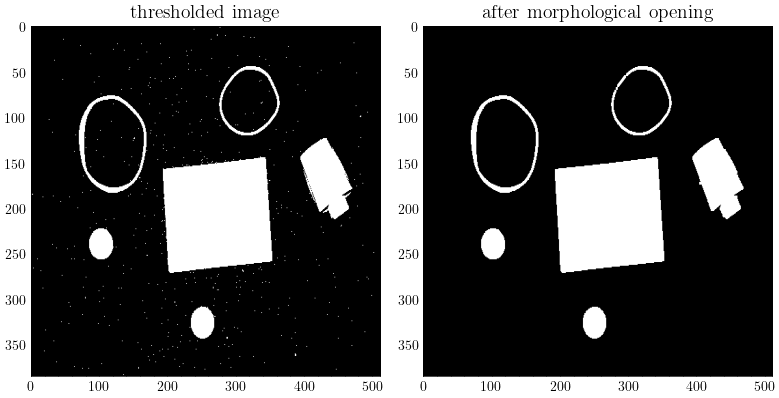
\includegraphics[width=0.8\textwidth]{figures/task_5_1.png}
    \caption{Cleaning up binary segmentation using morphological opening.}
    \label{fig:5.1}
\end{figure}

By visual inspection, the result is nearly perfect for all but the green object,
which has lost a small amount of detail from its outline as a result of the
opening. This is shown in \cref{fig:5.1_b}.

\begin{figure}[h]
    \centering
    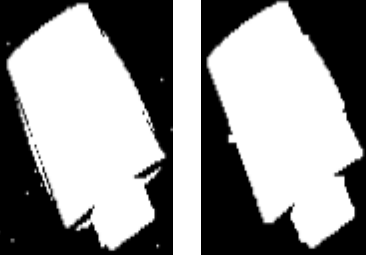
\includegraphics[width=0.4\textwidth]{figures/task_5_1_b.png}
    \caption{Close-up of segmentation of the green object before and after
    morphological opening.}
    \label{fig:5.1_b}
\end{figure}
